\section{Introduction}
\label{sec:introduction}

Consider four known query tokens at positions 765--768. Batching them exposes parallel work and weight reuse. At a KV-cache padding boundary, a wider call can enlarge earlier queries' physical attention ranges. The causal mask hides the same future tokens, yet output bytes can change. Query width can also select a different activation quantizer or dot-product specialization. The inputs are already available as a prompt suffix or a seed followed by draft proposals; grouping them requires no prediction of a causally unknown token.

Existing software can depend on a numerical path. A regression test compares complete output vectors; an exact replay resumes stored cache state; a replacement component hands state to an unchanged consumer. These settings fix the reference before optimization. We ask: \emph{what parallel execution remains available under that constraint?}

Several approaches already provide deterministic inference. Batch-invariant kernels make numerical results insensitive to batch composition~\cite{thinkingmachines}. Fixed scheduling makes selected execution shapes repeatable~\cite{corun}. Verified speculation uses a consistent verifier to repair a fast path and its KV state~\cite{llm42}. Arithmetic reconstruction also shows that output tiling and pipelining can change while a GPU kernel retains its per-output computation~\cite{taming}. The question here is how to apply that execution freedom within a quantized decoder whose query-specific numerical path is already chosen. We retain that path while changing the placement of attention cuts and the organization of independent projection groups.

The construction separates two grouping decisions. A \emph{physical run} contains adjacent queries that can share the reference's attention range and descriptor. An \emph{arithmetic group} retains a projection's column width, activation quantization and reduction organization. The boundaries can differ: attention may need a cut inside a group of projections that remains compatible when evaluated together. Keeping that cut inside attention preserves wider surrounding work. Exposing several compatible arithmetic groups through an outer tensor dimension provides another source of parallelism. The executor then restores the logical output order and commits the accepted cache prefix together with the consumer's token state (Fig.~\ref{fig:overview}).

\begin{figure*}[t]
 \centering
 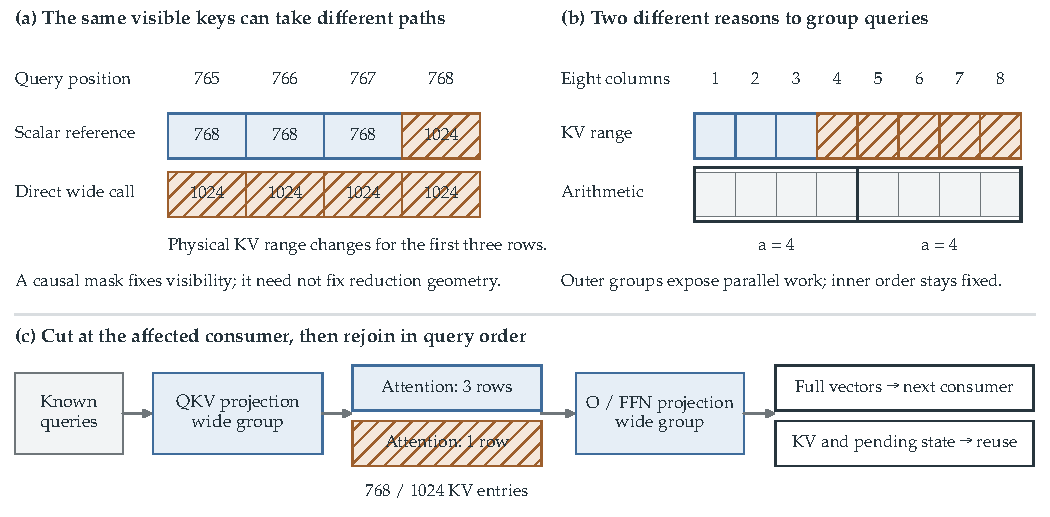
\includegraphics[width=\textwidth]{fig01_overview.pdf}
 \caption{Retain each group's numerical path while reorganizing execution across groups. (a) Four known queries cross a physical KV boundary. (b) Whole-call cuts divide surrounding projections; local cuts retain one four-column projection group while splitting attention. The backend must preserve the reference for each employed one- to four-column path. (c) Owned outputs retain row order; accepting two proposals keeps KV through position 767, while the correction at 768 remains pending. (d) A separate eight-query prefill illustrates two four-column arithmetic groups and attention tiles of four, three and one. Conceptual diagram prepared with ChatGPT (OpenAI, GPT-6 Astra Pro) assistance; editable drawing code is supplied.}
 \label{fig:overview}
\end{figure*}

This organization reuses existing small-column kernels, packing, weight broadcasting and fixed reductions. Its contribution is the construction that combines their arithmetic requirements with physical attention ranges and downstream output/state obligations. Structural invariants make the row mapping and cut placement explicit; backend conditions state what must hold for the arithmetic; qualification checks those conditions' consequences in the evaluated implementations. A conditional composition argument connects the resulting operations to subsequent decoder calls.

The experiments separate the method's two mechanisms and the costs around them. The 32B mixed-quantization instance keeps one-column arithmetic and whole-call cuts, isolating independent-group scheduling. Against a backend scalar loop that already shares activation quantization, it reduces A5000 target-only resident-service time by 1.51\% (95\% paired-root interval: 1.23--1.79\%). Q8 factorials independently vary four-column projection packing and whole versus local attention cuts. Controlled Vulkan appends measure the benefit of crossing a physical boundary; natural requests measure how often that opportunity occurs. Width experiments then show how cheaper equal-work verification can coexist with higher service time when deeper speculation creates extra target and draft work.

The paper contributes:
\begin{enumerate}
 \item A construction for fixed-reference parallel execution that separates physical and arithmetic groups, locates attention cuts, and preserves requested outputs and successor state.
 \item Concrete scalar-column and four-column CUDA instances, together with a Vulkan local-cut study, that connect the construction to existing quantized kernels and fair controls.
 \item An explanation of performance through grouping opportunities and their costs, supported by strong-control comparisons, component attribution, application measurements and negative cases.
\end{enumerate}
